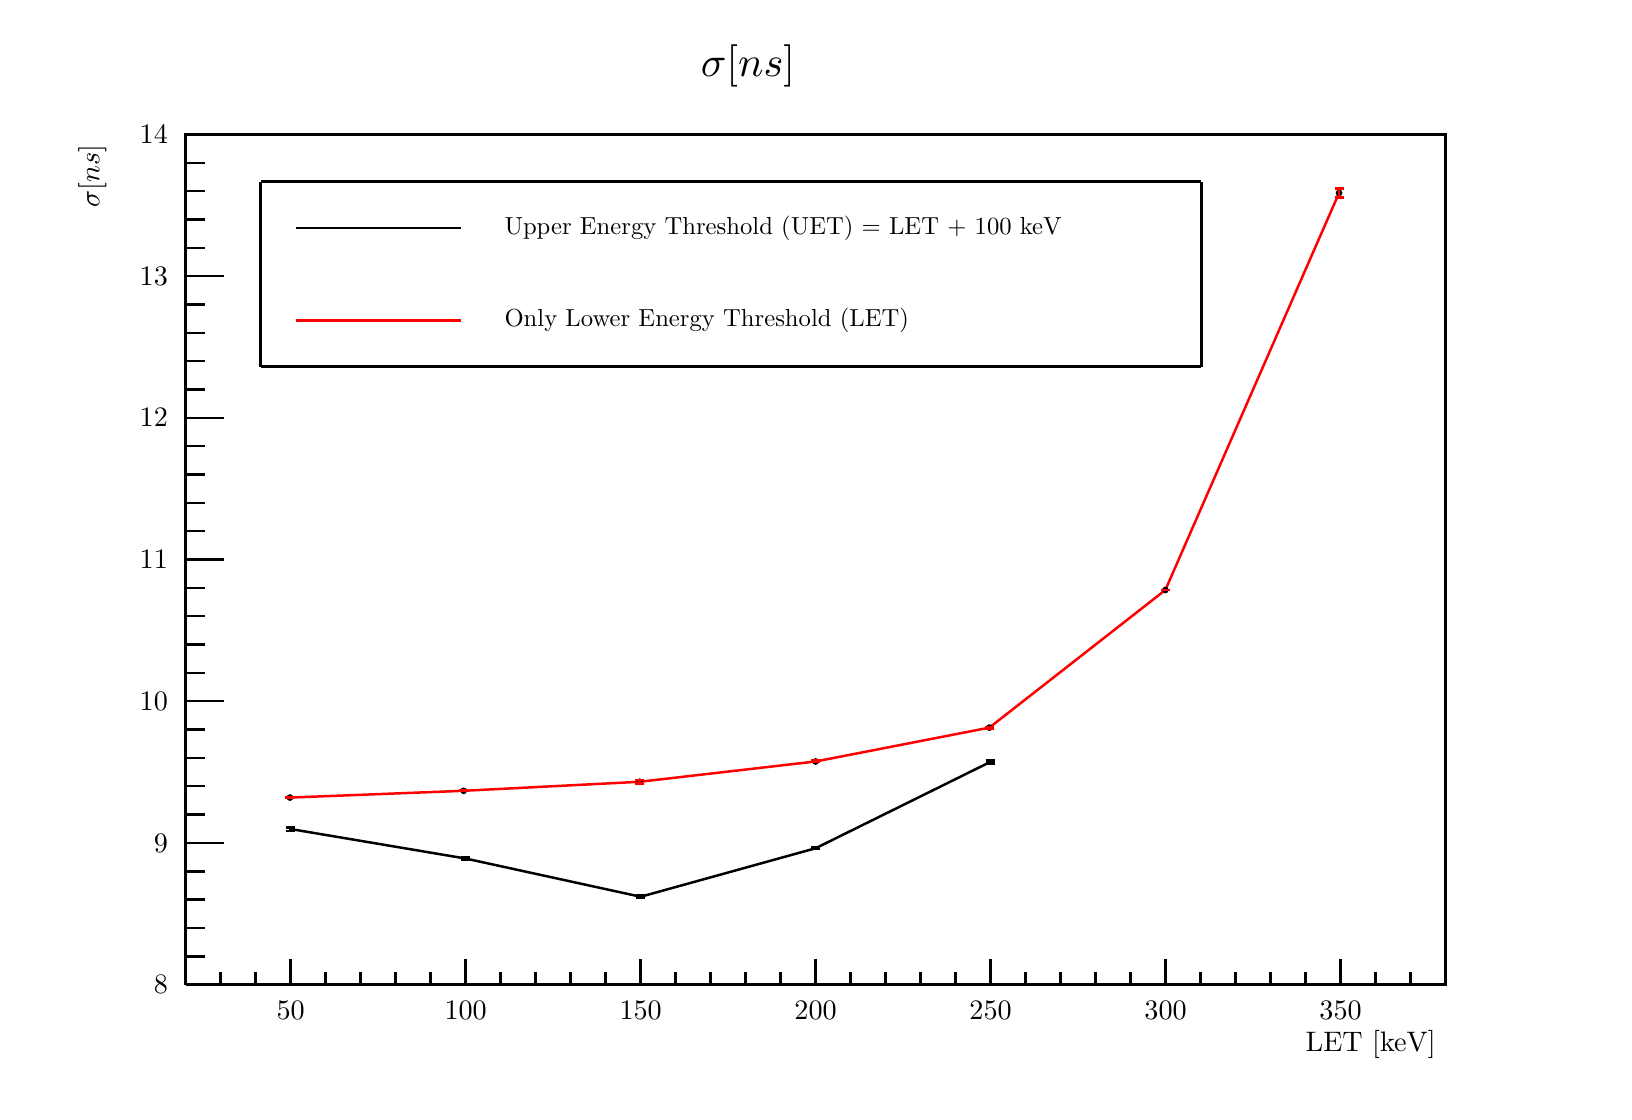
\begin{tikzpicture}
\pgfdeclareplotmark{cross} {
\pgfpathmoveto{\pgfpoint{-0.3\pgfplotmarksize}{\pgfplotmarksize}}
\pgfpathlineto{\pgfpoint{+0.3\pgfplotmarksize}{\pgfplotmarksize}}
\pgfpathlineto{\pgfpoint{+0.3\pgfplotmarksize}{0.3\pgfplotmarksize}}
\pgfpathlineto{\pgfpoint{+1\pgfplotmarksize}{0.3\pgfplotmarksize}}
\pgfpathlineto{\pgfpoint{+1\pgfplotmarksize}{-0.3\pgfplotmarksize}}
\pgfpathlineto{\pgfpoint{+0.3\pgfplotmarksize}{-0.3\pgfplotmarksize}}
\pgfpathlineto{\pgfpoint{+0.3\pgfplotmarksize}{-1.\pgfplotmarksize}}
\pgfpathlineto{\pgfpoint{-0.3\pgfplotmarksize}{-1.\pgfplotmarksize}}
\pgfpathlineto{\pgfpoint{-0.3\pgfplotmarksize}{-0.3\pgfplotmarksize}}
\pgfpathlineto{\pgfpoint{-1.\pgfplotmarksize}{-0.3\pgfplotmarksize}}
\pgfpathlineto{\pgfpoint{-1.\pgfplotmarksize}{0.3\pgfplotmarksize}}
\pgfpathlineto{\pgfpoint{-0.3\pgfplotmarksize}{0.3\pgfplotmarksize}}
\pgfpathclose
\pgfusepathqstroke
}
\pgfdeclareplotmark{cross*} {
\pgfpathmoveto{\pgfpoint{-0.3\pgfplotmarksize}{\pgfplotmarksize}}
\pgfpathlineto{\pgfpoint{+0.3\pgfplotmarksize}{\pgfplotmarksize}}
\pgfpathlineto{\pgfpoint{+0.3\pgfplotmarksize}{0.3\pgfplotmarksize}}
\pgfpathlineto{\pgfpoint{+1\pgfplotmarksize}{0.3\pgfplotmarksize}}
\pgfpathlineto{\pgfpoint{+1\pgfplotmarksize}{-0.3\pgfplotmarksize}}
\pgfpathlineto{\pgfpoint{+0.3\pgfplotmarksize}{-0.3\pgfplotmarksize}}
\pgfpathlineto{\pgfpoint{+0.3\pgfplotmarksize}{-1.\pgfplotmarksize}}
\pgfpathlineto{\pgfpoint{-0.3\pgfplotmarksize}{-1.\pgfplotmarksize}}
\pgfpathlineto{\pgfpoint{-0.3\pgfplotmarksize}{-0.3\pgfplotmarksize}}
\pgfpathlineto{\pgfpoint{-1.\pgfplotmarksize}{-0.3\pgfplotmarksize}}
\pgfpathlineto{\pgfpoint{-1.\pgfplotmarksize}{0.3\pgfplotmarksize}}
\pgfpathlineto{\pgfpoint{-0.3\pgfplotmarksize}{0.3\pgfplotmarksize}}
\pgfpathclose
\pgfusepathqfillstroke
}
\pgfdeclareplotmark{newstar} {
\pgfpathmoveto{\pgfqpoint{0pt}{\pgfplotmarksize}}
\pgfpathlineto{\pgfqpointpolar{44}{0.5\pgfplotmarksize}}
\pgfpathlineto{\pgfqpointpolar{18}{\pgfplotmarksize}}
\pgfpathlineto{\pgfqpointpolar{-20}{0.5\pgfplotmarksize}}
\pgfpathlineto{\pgfqpointpolar{-54}{\pgfplotmarksize}}
\pgfpathlineto{\pgfqpointpolar{-90}{0.5\pgfplotmarksize}}
\pgfpathlineto{\pgfqpointpolar{234}{\pgfplotmarksize}}
\pgfpathlineto{\pgfqpointpolar{198}{0.5\pgfplotmarksize}}
\pgfpathlineto{\pgfqpointpolar{162}{\pgfplotmarksize}}
\pgfpathlineto{\pgfqpointpolar{134}{0.5\pgfplotmarksize}}
\pgfpathclose
\pgfusepathqstroke
}
\pgfdeclareplotmark{newstar*} {
\pgfpathmoveto{\pgfqpoint{0pt}{\pgfplotmarksize}}
\pgfpathlineto{\pgfqpointpolar{44}{0.5\pgfplotmarksize}}
\pgfpathlineto{\pgfqpointpolar{18}{\pgfplotmarksize}}
\pgfpathlineto{\pgfqpointpolar{-20}{0.5\pgfplotmarksize}}
\pgfpathlineto{\pgfqpointpolar{-54}{\pgfplotmarksize}}
\pgfpathlineto{\pgfqpointpolar{-90}{0.5\pgfplotmarksize}}
\pgfpathlineto{\pgfqpointpolar{234}{\pgfplotmarksize}}
\pgfpathlineto{\pgfqpointpolar{198}{0.5\pgfplotmarksize}}
\pgfpathlineto{\pgfqpointpolar{162}{\pgfplotmarksize}}
\pgfpathlineto{\pgfqpointpolar{134}{0.5\pgfplotmarksize}}
\pgfpathclose
\pgfusepathqfillstroke
}
\definecolor{c}{rgb}{1,1,1};
\draw [color=c, fill=c] (0,0) rectangle (20,13.4957);
\draw [color=c, fill=c] (2,1.34957) rectangle (18,12.1461);
\definecolor{c}{rgb}{0,0,0};
\draw [c,line width=0.9] (2,1.34957) -- (2,12.1461) -- (18,12.1461) -- (18,1.34957) -- (2,1.34957);
\definecolor{c}{rgb}{1,1,1};
\draw [color=c, fill=c] (2,1.34957) rectangle (18,12.1461);
\definecolor{c}{rgb}{0,0,0};
\draw [c,line width=0.9] (2,1.34957) -- (2,12.1461) -- (18,12.1461) -- (18,1.34957) -- (2,1.34957);
\draw [c,line width=0.9] (2,1.34957) -- (18,1.34957);
\draw [c,line width=0.9] (3.33333,1.67347) -- (3.33333,1.34957);
\draw [c,line width=0.9] (3.77778,1.51152) -- (3.77778,1.34957);
\draw [c,line width=0.9] (4.22222,1.51152) -- (4.22222,1.34957);
\draw [c,line width=0.9] (4.66667,1.51152) -- (4.66667,1.34957);
\draw [c,line width=0.9] (5.11111,1.51152) -- (5.11111,1.34957);
\draw [c,line width=0.9] (5.55556,1.67347) -- (5.55556,1.34957);
\draw [c,line width=0.9] (6,1.51152) -- (6,1.34957);
\draw [c,line width=0.9] (6.44444,1.51152) -- (6.44444,1.34957);
\draw [c,line width=0.9] (6.88889,1.51152) -- (6.88889,1.34957);
\draw [c,line width=0.9] (7.33333,1.51152) -- (7.33333,1.34957);
\draw [c,line width=0.9] (7.77778,1.67347) -- (7.77778,1.34957);
\draw [c,line width=0.9] (8.22222,1.51152) -- (8.22222,1.34957);
\draw [c,line width=0.9] (8.66667,1.51152) -- (8.66667,1.34957);
\draw [c,line width=0.9] (9.11111,1.51152) -- (9.11111,1.34957);
\draw [c,line width=0.9] (9.55556,1.51152) -- (9.55556,1.34957);
\draw [c,line width=0.9] (10,1.67347) -- (10,1.34957);
\draw [c,line width=0.9] (10.4444,1.51152) -- (10.4444,1.34957);
\draw [c,line width=0.9] (10.8889,1.51152) -- (10.8889,1.34957);
\draw [c,line width=0.9] (11.3333,1.51152) -- (11.3333,1.34957);
\draw [c,line width=0.9] (11.7778,1.51152) -- (11.7778,1.34957);
\draw [c,line width=0.9] (12.2222,1.67347) -- (12.2222,1.34957);
\draw [c,line width=0.9] (12.6667,1.51152) -- (12.6667,1.34957);
\draw [c,line width=0.9] (13.1111,1.51152) -- (13.1111,1.34957);
\draw [c,line width=0.9] (13.5556,1.51152) -- (13.5556,1.34957);
\draw [c,line width=0.9] (14,1.51152) -- (14,1.34957);
\draw [c,line width=0.9] (14.4444,1.67347) -- (14.4444,1.34957);
\draw [c,line width=0.9] (14.8889,1.51152) -- (14.8889,1.34957);
\draw [c,line width=0.9] (15.3333,1.51152) -- (15.3333,1.34957);
\draw [c,line width=0.9] (15.7778,1.51152) -- (15.7778,1.34957);
\draw [c,line width=0.9] (16.2222,1.51152) -- (16.2222,1.34957);
\draw [c,line width=0.9] (16.6667,1.67347) -- (16.6667,1.34957);
\draw [c,line width=0.9] (3.33333,1.67347) -- (3.33333,1.34957);
\draw [c,line width=0.9] (2.88889,1.51152) -- (2.88889,1.34957);
\draw [c,line width=0.9] (2.44444,1.51152) -- (2.44444,1.34957);
\draw [c,line width=0.9] (16.6667,1.67347) -- (16.6667,1.34957);
\draw [c,line width=0.9] (17.1111,1.51152) -- (17.1111,1.34957);
\draw [c,line width=0.9] (17.5556,1.51152) -- (17.5556,1.34957);
\draw [c,line width=0.9] (18,1.51152) -- (18,1.34957);
\draw [anchor=base] (3.33333,0.904212) node[scale=1.01821, color=c, rotate=0]{50};
\draw [anchor=base] (5.55556,0.904212) node[scale=1.01821, color=c, rotate=0]{100};
\draw [anchor=base] (7.77778,0.904212) node[scale=1.01821, color=c, rotate=0]{150};
\draw [anchor=base] (10,0.904212) node[scale=1.01821, color=c, rotate=0]{200};
\draw [anchor=base] (12.2222,0.904212) node[scale=1.01821, color=c, rotate=0]{250};
\draw [anchor=base] (14.4444,0.904212) node[scale=1.01821, color=c, rotate=0]{300};
\draw [anchor=base] (16.6667,0.904212) node[scale=1.01821, color=c, rotate=0]{350};
\draw [anchor= east] (18,0.593811) node[scale=1.01821, color=c, rotate=0]{LET [keV]};
\draw [c,line width=0.9] (2,1.34957) -- (2,12.1461);
\draw [c,line width=0.9] (2.48,1.34957) -- (2,1.34957);
\draw [c,line width=0.9] (2.24,1.70946) -- (2,1.70946);
\draw [c,line width=0.9] (2.24,2.06934) -- (2,2.06934);
\draw [c,line width=0.9] (2.24,2.42923) -- (2,2.42923);
\draw [c,line width=0.9] (2.24,2.78911) -- (2,2.78911);
\draw [c,line width=0.9] (2.48,3.149) -- (2,3.149);
\draw [c,line width=0.9] (2.24,3.50888) -- (2,3.50888);
\draw [c,line width=0.9] (2.24,3.86877) -- (2,3.86877);
\draw [c,line width=0.9] (2.24,4.22865) -- (2,4.22865);
\draw [c,line width=0.9] (2.24,4.58854) -- (2,4.58854);
\draw [c,line width=0.9] (2.48,4.94842) -- (2,4.94842);
\draw [c,line width=0.9] (2.24,5.30831) -- (2,5.30831);
\draw [c,line width=0.9] (2.24,5.66819) -- (2,5.66819);
\draw [c,line width=0.9] (2.24,6.02808) -- (2,6.02808);
\draw [c,line width=0.9] (2.24,6.38797) -- (2,6.38797);
\draw [c,line width=0.9] (2.48,6.74785) -- (2,6.74785);
\draw [c,line width=0.9] (2.24,7.10774) -- (2,7.10774);
\draw [c,line width=0.9] (2.24,7.46762) -- (2,7.46762);
\draw [c,line width=0.9] (2.24,7.82751) -- (2,7.82751);
\draw [c,line width=0.9] (2.24,8.18739) -- (2,8.18739);
\draw [c,line width=0.9] (2.48,8.54728) -- (2,8.54728);
\draw [c,line width=0.9] (2.24,8.90716) -- (2,8.90716);
\draw [c,line width=0.9] (2.24,9.26705) -- (2,9.26705);
\draw [c,line width=0.9] (2.24,9.62693) -- (2,9.62693);
\draw [c,line width=0.9] (2.24,9.98682) -- (2,9.98682);
\draw [c,line width=0.9] (2.48,10.3467) -- (2,10.3467);
\draw [c,line width=0.9] (2.24,10.7066) -- (2,10.7066);
\draw [c,line width=0.9] (2.24,11.0665) -- (2,11.0665);
\draw [c,line width=0.9] (2.24,11.4264) -- (2,11.4264);
\draw [c,line width=0.9] (2.24,11.7862) -- (2,11.7862);
\draw [c,line width=0.9] (2.48,12.1461) -- (2,12.1461);
\draw [anchor= east] (1.9,1.34957) node[scale=1.01821, color=c, rotate=0]{8};
\draw [anchor= east] (1.9,3.149) node[scale=1.01821, color=c, rotate=0]{9};
\draw [anchor= east] (1.9,4.94842) node[scale=1.01821, color=c, rotate=0]{10};
\draw [anchor= east] (1.9,6.74785) node[scale=1.01821, color=c, rotate=0]{11};
\draw [anchor= east] (1.9,8.54728) node[scale=1.01821, color=c, rotate=0]{12};
\draw [anchor= east] (1.9,10.3467) node[scale=1.01821, color=c, rotate=0]{13};
\draw [anchor= east] (1.9,12.1461) node[scale=1.01821, color=c, rotate=0]{14};
\draw [anchor= east] (0.812894,12.1461) node[scale=1.01821, color=c, rotate=90]{$\sigma [ns]$};
\definecolor{c}{rgb}{1,0,0};
\draw [c,line width=0.9] (3.32378,3.72493) -- (5.53009,3.81089) -- (7.76504,3.9255) -- (10,4.18338) -- (12.2063,4.61318) -- (14.4413,6.36103) -- (16.6476,11.404);
\definecolor{c}{rgb}{0,0,0};
\foreach \P in {(3.32378,3.72493), (5.53009,3.81089), (7.76504,3.9255), (10,4.18338), (12.2063,4.61318), (14.4413,6.36103), (16.6476,11.404)}{\draw[mark options={color=c,fill=c},mark size=2.402402pt,mark=*,mark size=1pt] plot coordinates {\P};}
\definecolor{c}{rgb}{1,0,0};
\draw [c,line width=0.9] (3.32378,3.72493) -- (3.32378,3.72743);
\draw [c,line width=0.9] (3.26648,3.72743) -- (3.38109,3.72743);
\draw [c,line width=0.9] (3.32378,3.72493) -- (3.32378,3.72242);
\draw [c,line width=0.9] (3.26648,3.72242) -- (3.38109,3.72242);
\draw [c,line width=0.9] (5.53009,3.81089) -- (5.53009,3.81168);
\draw [c,line width=0.9] (5.47278,3.81168) -- (5.58739,3.81168);
\draw [c,line width=0.9] (5.53009,3.81089) -- (5.53009,3.8101);
\draw [c,line width=0.9] (5.47278,3.8101) -- (5.58739,3.8101);
\draw [c,line width=0.9] (7.76504,3.9255) -- (7.76504,3.95001);
\draw [c,line width=0.9] (7.70774,3.95001) -- (7.82235,3.95001);
\draw [c,line width=0.9] (7.76504,3.9255) -- (7.76504,3.90099);
\draw [c,line width=0.9] (7.70774,3.90099) -- (7.82235,3.90099);
\draw [c,line width=0.9] (10,4.18338) -- (10,4.19299);
\draw [c,line width=0.9] (9.94269,4.19299) -- (10.0573,4.19299);
\draw [c,line width=0.9] (10,4.18338) -- (10,4.17378);
\draw [c,line width=0.9] (9.94269,4.17378) -- (10.0573,4.17378);
\draw [c,line width=0.9] (12.2063,4.61318) -- (12.2063,4.62252);
\draw [c,line width=0.9] (12.149,4.62252) -- (12.2636,4.62252);
\draw [c,line width=0.9] (12.2063,4.61318) -- (12.2063,4.60384);
\draw [c,line width=0.9] (12.149,4.60384) -- (12.2636,4.60384);
\draw [c,line width=0.9] (14.4413,6.36103) -- (14.4413,6.3631);
\draw [c,line width=0.9] (14.384,6.3631) -- (14.4986,6.3631);
\draw [c,line width=0.9] (14.4413,6.36103) -- (14.4413,6.35896);
\draw [c,line width=0.9] (14.384,6.35896) -- (14.4986,6.35896);
\draw [c,line width=0.9] (16.6476,11.404) -- (16.6476,11.4612);
\draw [c,line width=0.9] (16.5903,11.4612) -- (16.7049,11.4612);
\draw [c,line width=0.9] (16.6476,11.404) -- (16.6476,11.3468);
\draw [c,line width=0.9] (16.5903,11.3468) -- (16.7049,11.3468);
\definecolor{c}{rgb}{0,0,0};
\draw [c,line width=0.9] (3.33333,3.32529) -- (3.33333,3.34759);
\draw [c,line width=0.9] (3.27603,3.34759) -- (3.39064,3.34759);
\draw [c,line width=0.9] (3.33333,3.32529) -- (3.33333,3.30299);
\draw [c,line width=0.9] (3.27603,3.30299) -- (3.39064,3.30299);
\draw [c,line width=0.9] (5.55556,2.95054) -- (5.55556,2.96779);
\draw [c,line width=0.9] (5.49825,2.96779) -- (5.61286,2.96779);
\draw [c,line width=0.9] (5.55556,2.95054) -- (5.55556,2.93329);
\draw [c,line width=0.9] (5.49825,2.93329) -- (5.61286,2.93329);
\draw [c,line width=0.9] (7.77778,2.46539) -- (7.77778,2.47851);
\draw [c,line width=0.9] (7.72047,2.47851) -- (7.83508,2.47851);
\draw [c,line width=0.9] (7.77778,2.46539) -- (7.77778,2.45228);
\draw [c,line width=0.9] (7.72047,2.45228) -- (7.83508,2.45228);
\draw [c,line width=0.9] (10,3.08148) -- (10,3.08843);
\draw [c,line width=0.9] (9.94269,3.08843) -- (10.0573,3.08843);
\draw [c,line width=0.9] (10,3.08148) -- (10,3.07453);
\draw [c,line width=0.9] (9.94269,3.07453) -- (10.0573,3.07453);
\draw [c,line width=0.9] (12.2222,4.17955) -- (12.2222,4.19884);
\draw [c,line width=0.9] (12.1649,4.19884) -- (12.2795,4.19884);
\draw [c,line width=0.9] (12.2222,4.17955) -- (12.2222,4.16025);
\draw [c,line width=0.9] (12.1649,4.16025) -- (12.2795,4.16025);
\draw [c,line width=0.9] (3.33333,3.32529) -- (5.55556,2.95054) -- (7.77778,2.46539) -- (10,3.08148) -- (12.2222,4.17955);
\definecolor{c}{rgb}{1,1,1};
\draw [color=c, fill=c] (2.95129,9.19771) rectangle (14.8997,11.5473);
\definecolor{c}{rgb}{0,0,0};
\draw [c,line width=0.9] (2.95129,9.19771) -- (14.8997,9.19771);
\draw [c,line width=0.9] (14.8997,9.19771) -- (14.8997,11.5473);
\draw [c,line width=0.9] (14.8997,11.5473) -- (2.95129,11.5473);
\draw [c,line width=0.9] (2.95129,11.5473) -- (2.95129,9.19771);
\draw [anchor= west] (5.9384,10.9599) node[scale=0.890934, color=c, rotate=0]{Upper Energy Threshold (UET) = LET + 100 keV};
\draw [c,line width=0.9] (3.39936,10.9599) -- (5.49033,10.9599);
\draw [anchor= west] (5.9384,9.7851) node[scale=0.890934, color=c, rotate=0]{Only Lower Energy Threshold (LET)};
\definecolor{c}{rgb}{1,0,0};
\draw [c,line width=0.9] (3.39936,9.7851) -- (5.49033,9.7851);
\definecolor{c}{rgb}{0,0,0};
\draw (9.1404,13.0156) node[scale=1.52731, color=c, rotate=0]{$\sigma [ns]$};
\end{tikzpicture}
